\documentclass[10pt]{beamer}

\usepackage{setup}
\usepackage[vlined]{algorithm2e}
\SetAlFnt{\scriptsize}

\title{Time Warp Simulation on Multi-core Processors and Clusters}
\author{
    Douglas A. Weber \\
    Masters Thesis Defense \\
    Advisor: Professor Philip A. Wilsey
}
\institute{University of Cincinnati}
\date{March XX, 2016}

\begin{document}

\begin{frame}
  \titlepage
\end{frame}

\begin{frame}{Discrete Event Simulation}
    \begin{itemize}
        \item Three main components
            \begin{itemize}
                \item State variables
                \item Simulation clock
                \item Pending event set
            \end{itemize}
        \bigskip
        \item Unprocessed events stored in pending event set
        \item Events processed in time stamp order
        \item Simulation clock and state variables updated only when event occurs
    \end{itemize}
\end{frame}

\begin{frame}{Parallel Discrete Event Simulation}

    \begin{columns}[c]
    \begin{column}{0.4\textwidth}
        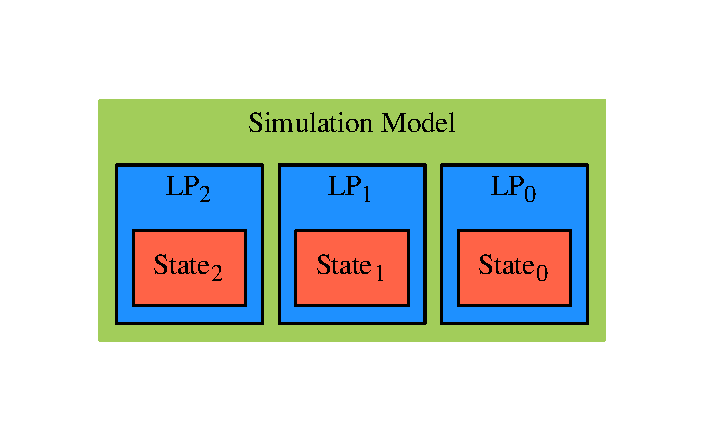
\includegraphics[width=\textwidth]{../figs/graphviz/pdes.pdf}
    \end{column}
    \begin{column}{0.6\textwidth}
        \begin{itemize}
            \item Model system as a set of Logical Processes (LPs)
            \item No shared state between LPs
        \end{itemize}
    \end{column}
    \end{columns}

    \begin{itemize}
        \item Events exchanged between LPs
    \end{itemize}

    \begin{block}{Possible Causality Violations}
        \begin{columns}[T]
        \begin{column}{0.4\textwidth}
            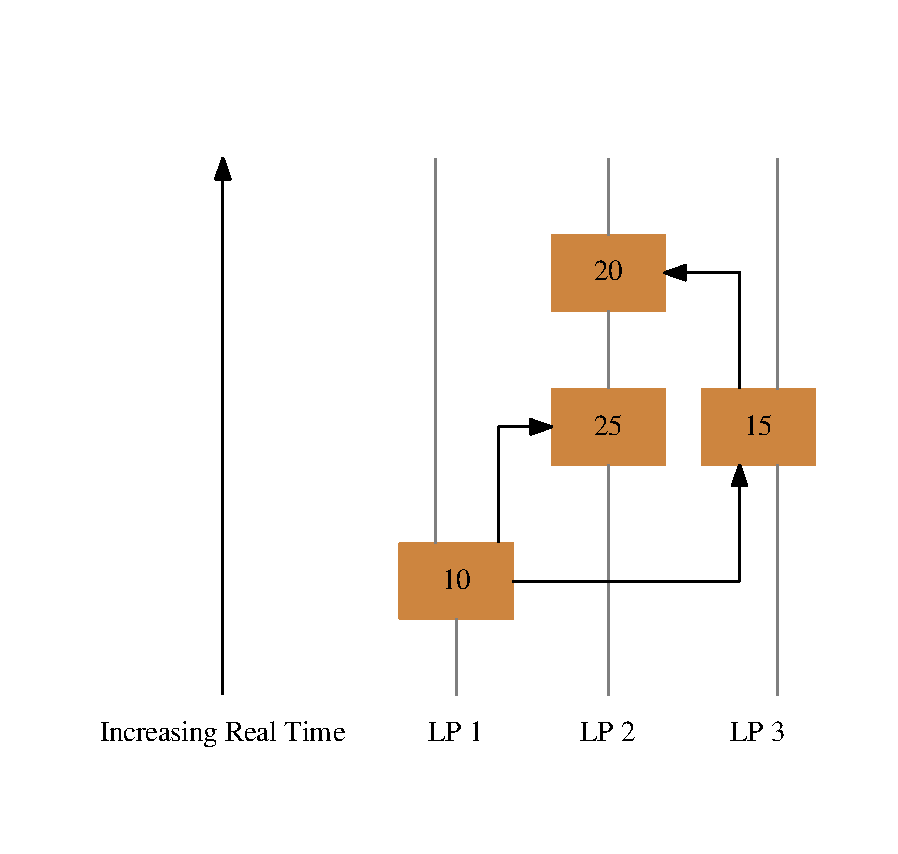
\includegraphics[width=\textwidth]{../figs/graphviz/causality.pdf}
        \end{column}
        \begin{column}{0.6\textwidth}
            \begin{itemize}
                \item Events can be received \& processed out of order
                \item Two solutions
                    \begin{itemize}
                        \item Conservative and Optimistic
                    \end{itemize}
            \end{itemize}
        \end{column}
    \end{columns}
    \end{block}

\end{frame}

\begin{frame}{Time Warp}
    \begin{block}{Optimistic Mechanism}
        \bigskip
        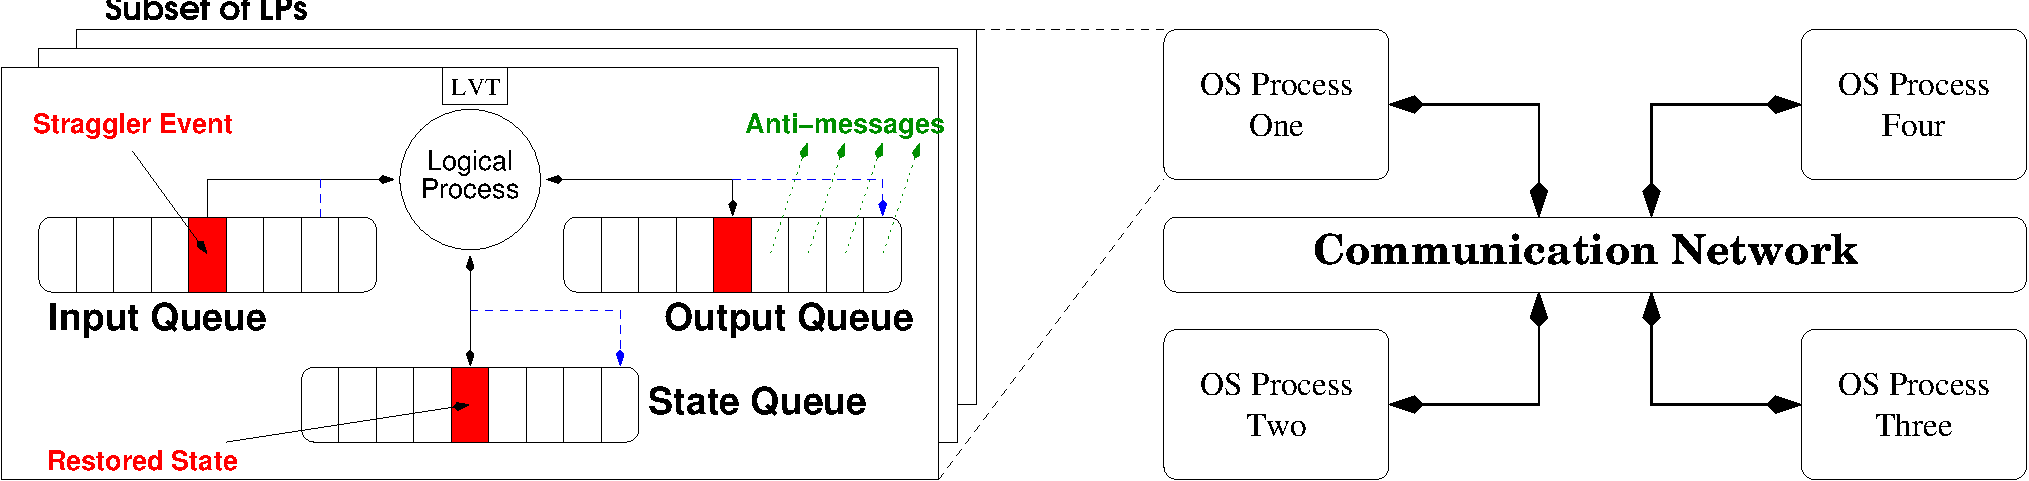
\includegraphics[width=\textwidth]{../figs/timeWarp.pdf}
        \bigskip
        \begin{itemize}
            \item Rollback Mechanism
                \begin{itemize}
                    \item State Restoration, Anti-Messages
                \end{itemize}
            \item Local Virtual Time (LVT) \& Global Virtual Time (GVT)
            \item Fossil Collection
        \end{itemize}
    \end{block}
\end{frame}

\begin{frame}{\textsc{warped2} Process}
        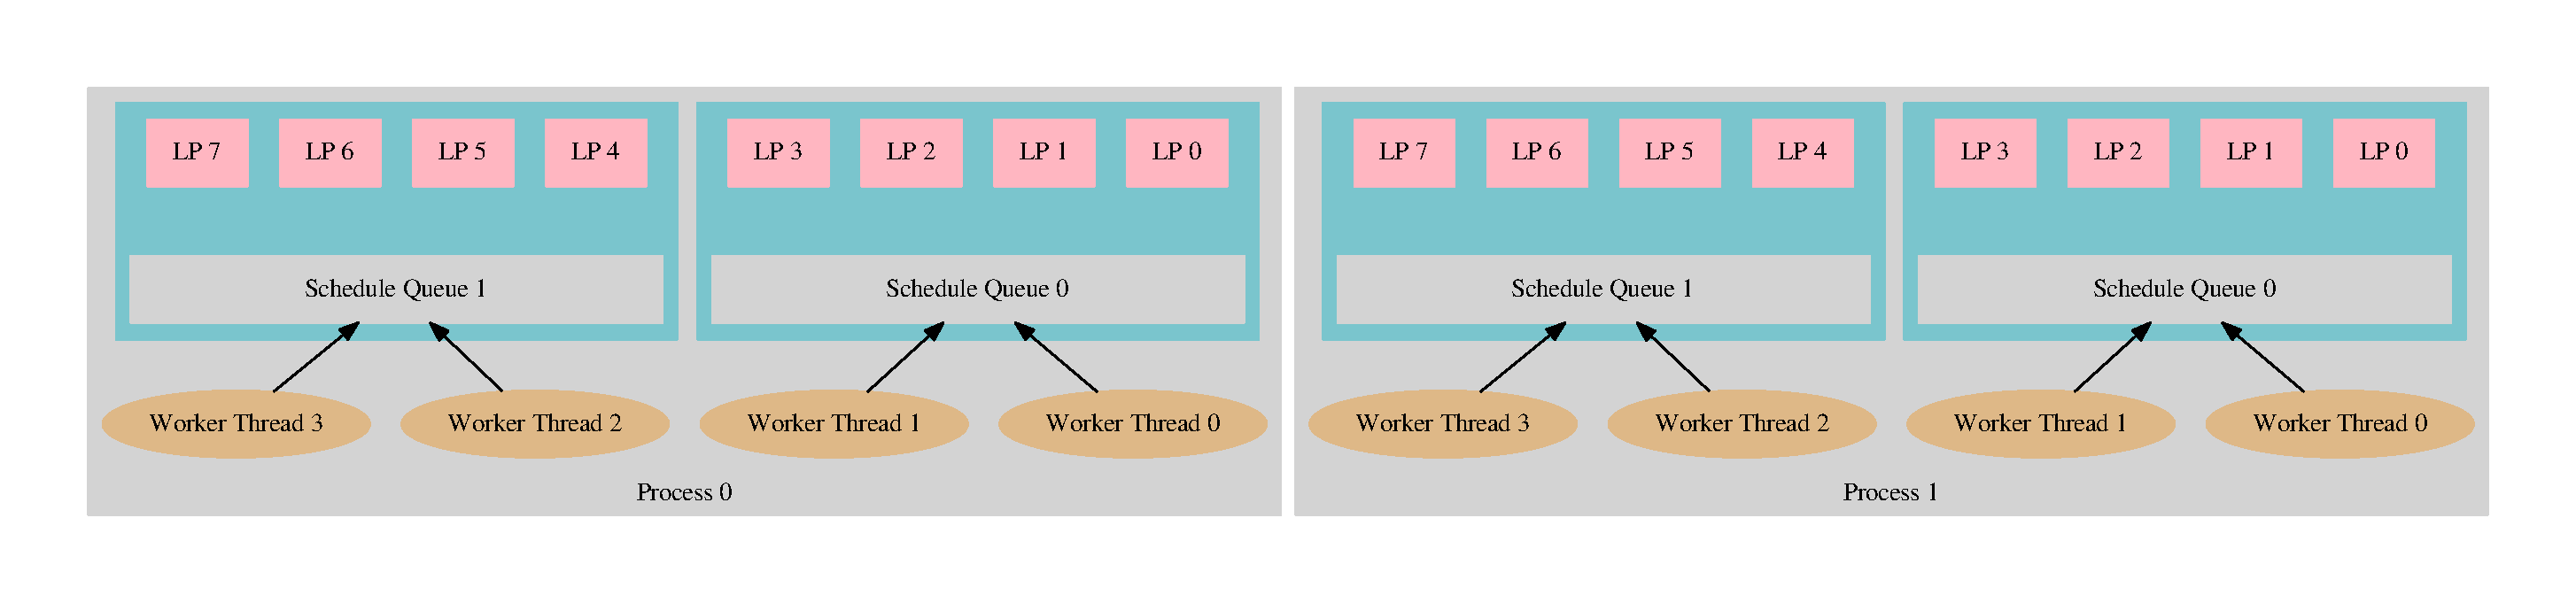
\includegraphics[width=\textwidth]{../figs/graphviz/partitioning.pdf}
        \begin{itemize}
            \item Worker Threads and Manager Thread
            \item LTSF Queues
            \item LP Partitioning
            \begin{itemize}
                \item Processes
                \item LTSF Queues
            \end{itemize}
        \end{itemize}
\end{frame}

\begin{frame}{Sharing LTSF Queues}
    \begin{minipage}{0.5\textwidth}
        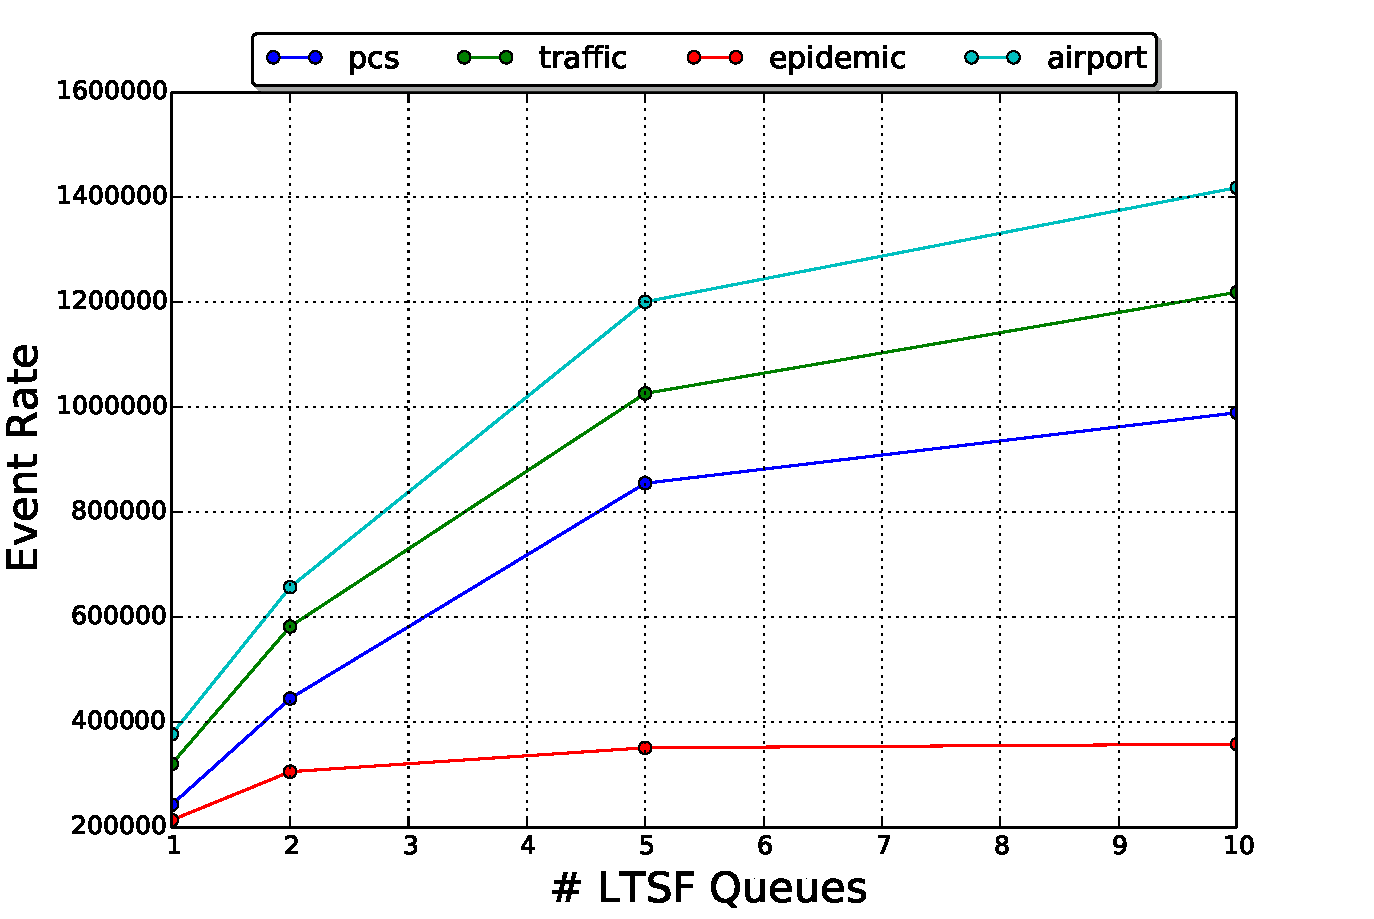
\includegraphics[width=\textwidth]{../figs/pending_event_set/ltsf_event_rate.pdf}
        $$EventRate={CommitedEvents \over Runtime}$$
    \end{minipage}%
    \begin{minipage}{0.5\textwidth}
        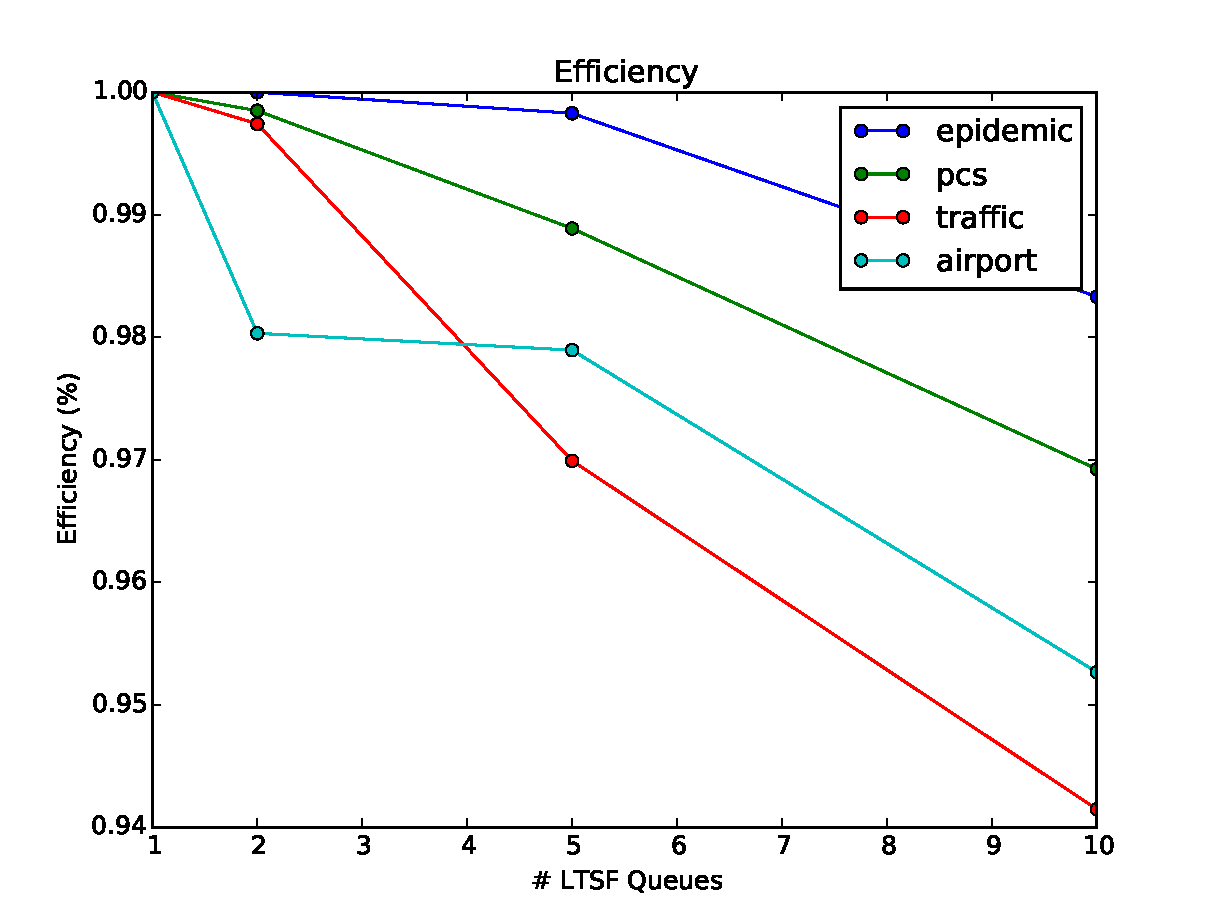
\includegraphics[width=\textwidth]{../figs/pending_event_set/ltsf_efficiency.pdf}
        $$Efficiency={CommittedEvents \over ProcessedEvents}*100 \%$$
    \end{minipage}
    \begin{block}{Reducing contention more important than reducing rollbacks}\end{block}
\end{frame}

\begin{frame}{Partitioning}
    \begin{center}
    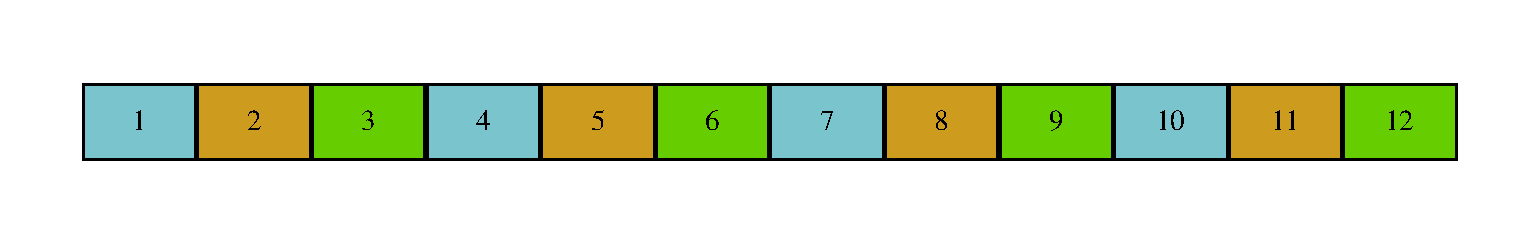
\includegraphics[width=0.8\textwidth]{../figs/graphviz/round_robin_partitioning.pdf} \\
    Round-Robin \\
    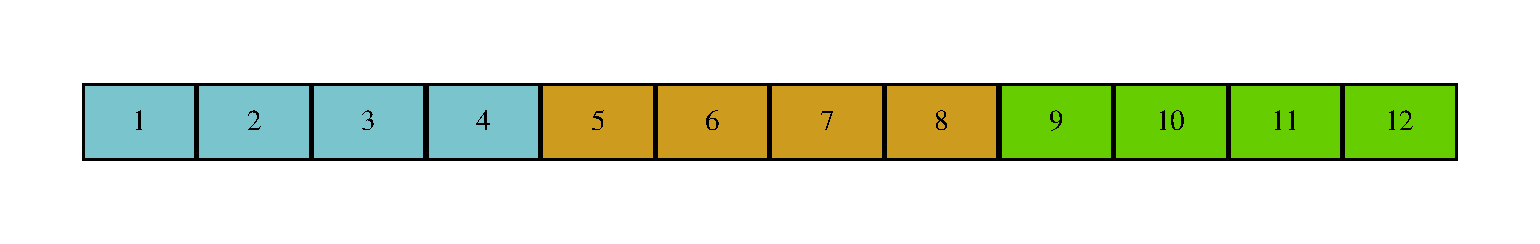
\includegraphics[width=0.8\textwidth]{../figs/graphviz/block_partitioning.pdf} \\
    Block \\
  \end{center}
\end{frame}

\begin{frame}{Periodic State Saving}
    \begin{block}{Save state only once every $N$ events}
        \begin{itemize}
            \item Not all states available to roll back to
            \item Must "Coast Forward" to reproduce state
            \item Decrease time to copy states and reduce memory footprint
            \item Increase rollback time
        \end{itemize}
    \end{block}
    \begin{block}{SMP Machine - Intel\textsuperscript{\textregistered} Xeon\textsuperscript{\textregistered} X5675}
        \smallskip
        \begin{minipage}{0.5\textwidth}
            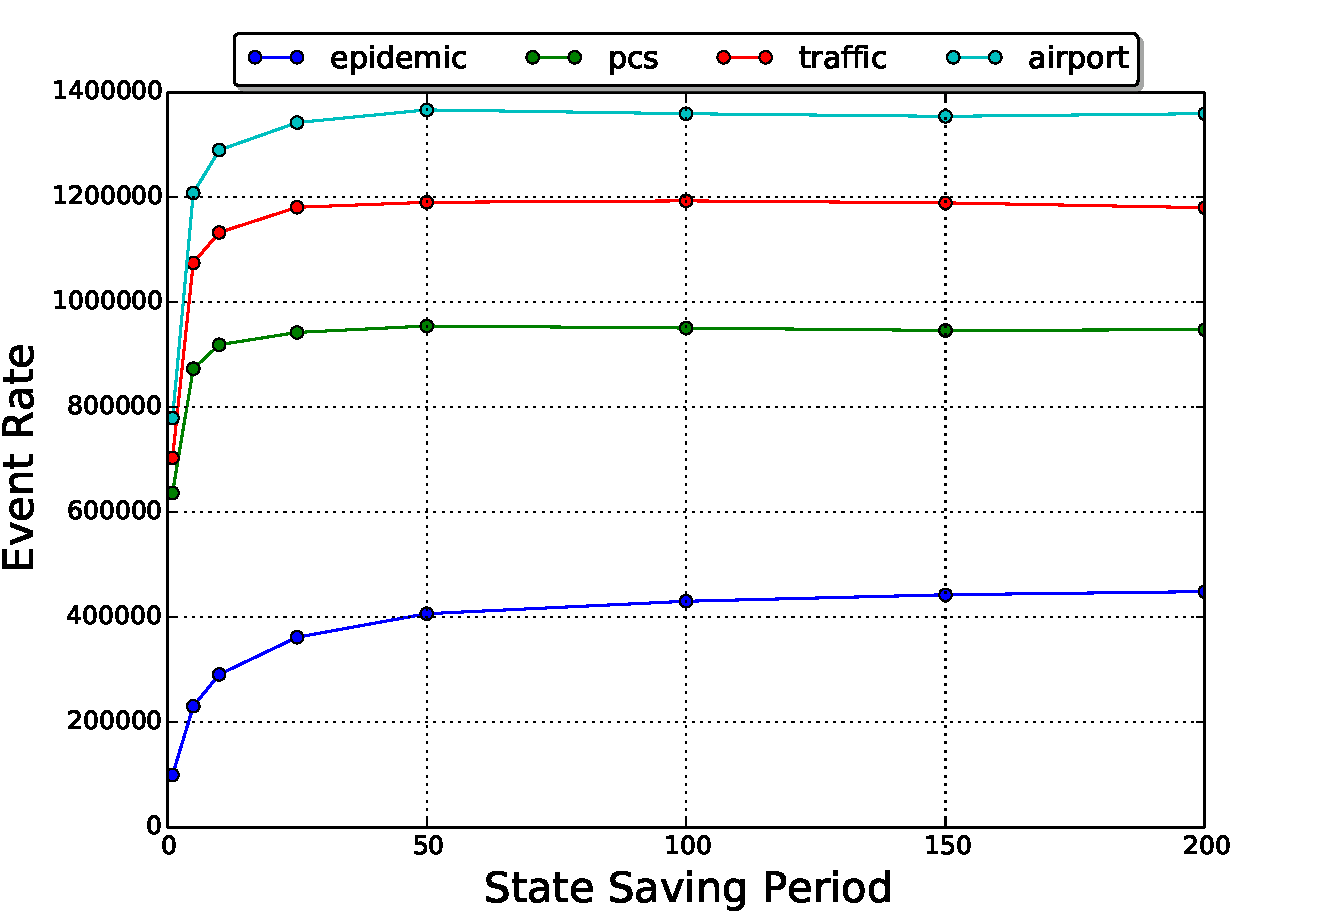
\includegraphics[width=\textwidth]{../figs/state_saving/bc/eventrate.pdf}
        \end{minipage}%
        \begin{minipage}{0.5\textwidth}
            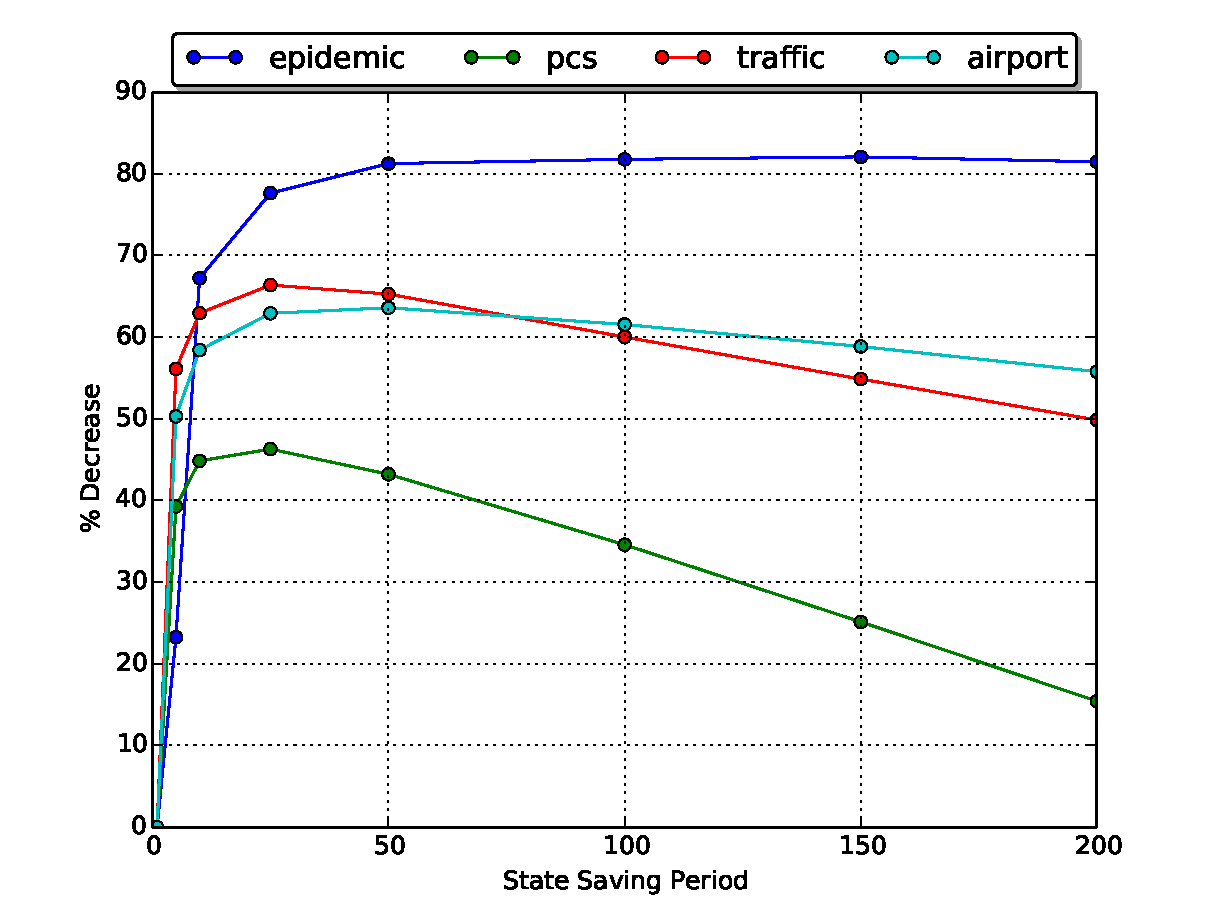
\includegraphics[width=\textwidth]{../figs/state_saving/bc/percent_memory_decrease.pdf}
        \end{minipage}
    \end{block}
\end{frame}

\begin{frame}{Periodic State Saving}
    \begin{block}{8 Node Cluster - Intel\textsuperscript{\textregistered} Xeon\textsuperscript{\textregistered} E5410}
        \smallskip
        \begin{minipage}{0.5\textwidth}
            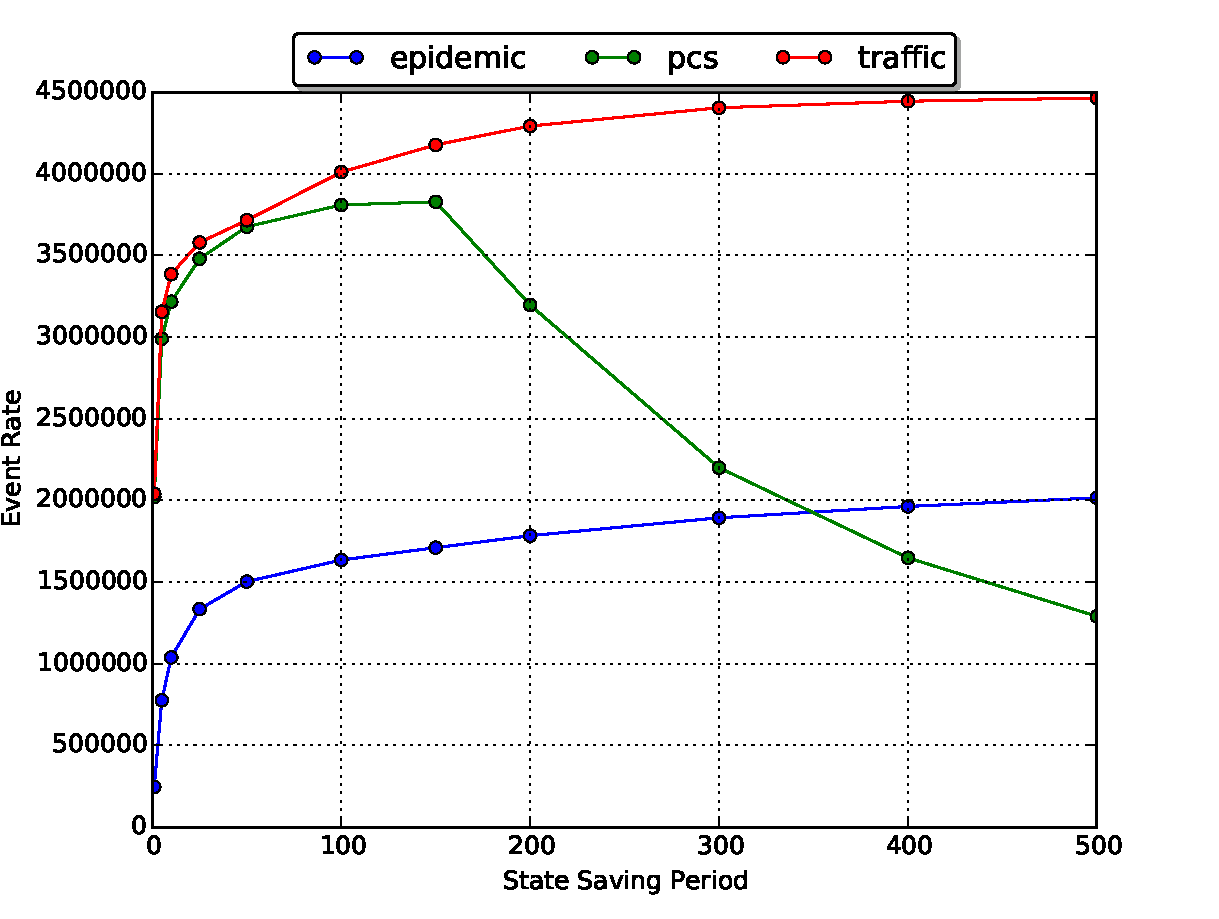
\includegraphics[width=\textwidth]{../figs/state_saving/beowulf/eventrate_500.pdf}
        \end{minipage}%
        \begin{minipage}{0.5\textwidth}
            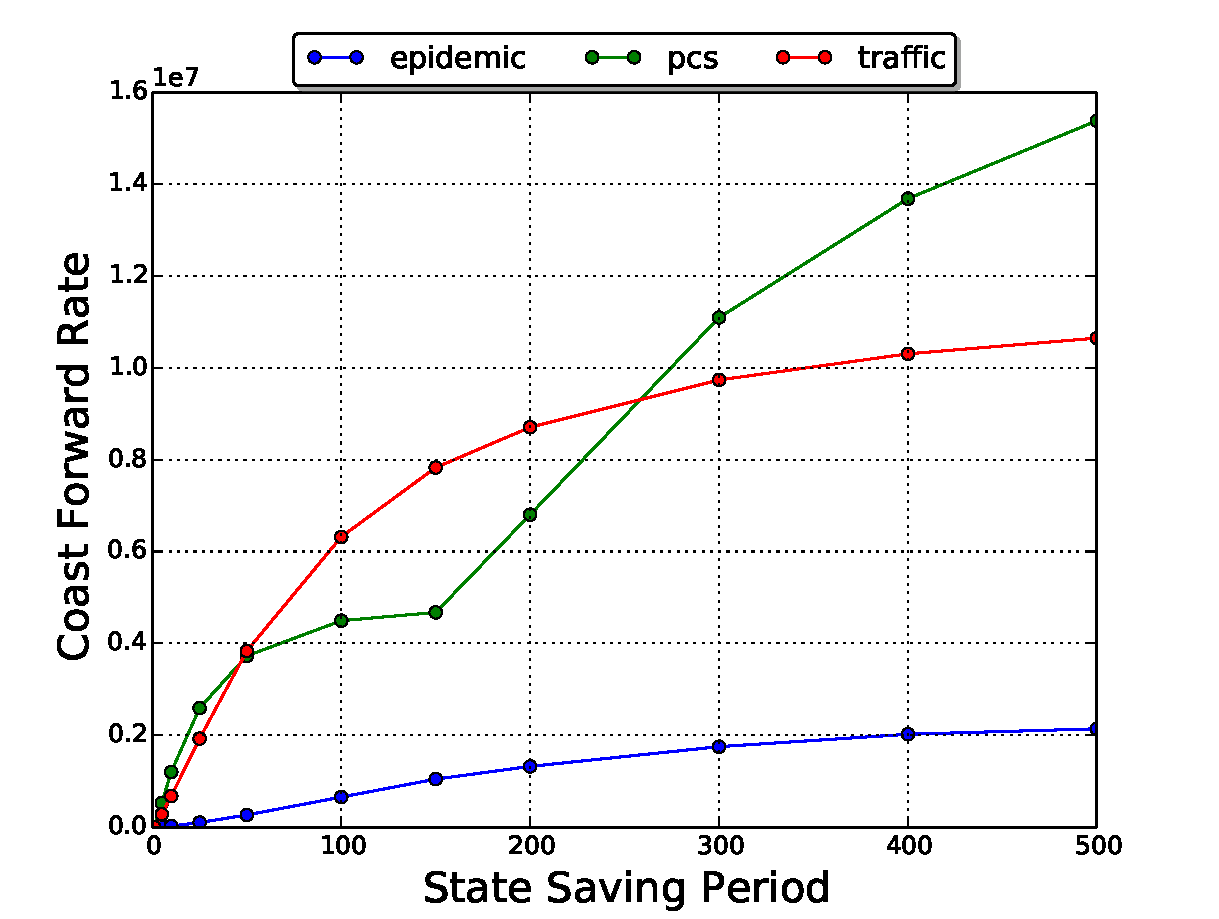
\includegraphics[width=\textwidth]{../figs/state_saving/beowulf/cf_rate_500.pdf}
        \end{minipage}
    $$ CoastForwardRate = {CoastForwardEvents \over Rollbacks} * RollbackRate $$
    \end{block}
\end{frame}

\begin{frame}{Memory Allocation}
    \begin{block}{SMP Machine - Intel\textsuperscript{\textregistered} Xeon\textsuperscript{\textregistered} X5675}
        \begin{columns}
        \begin{column}{0.5\textwidth}
            \smallskip
            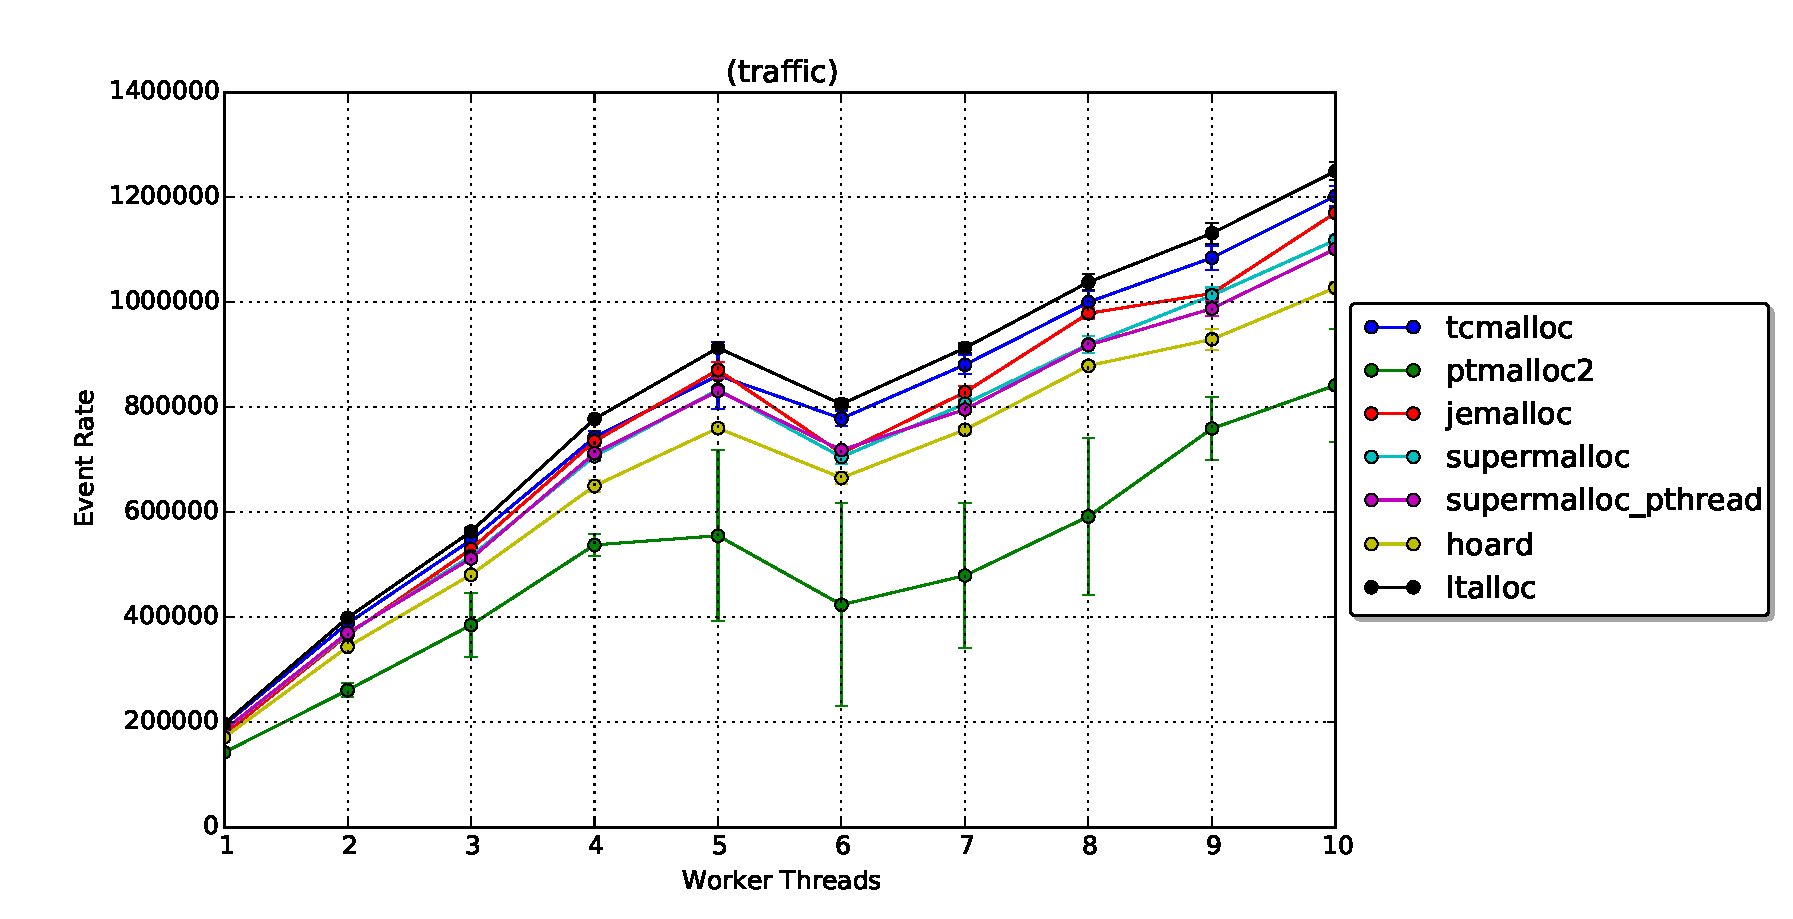
\includegraphics[width=\textwidth]{../figs/memory_allocation/traffic_eventrate.pdf} \\
            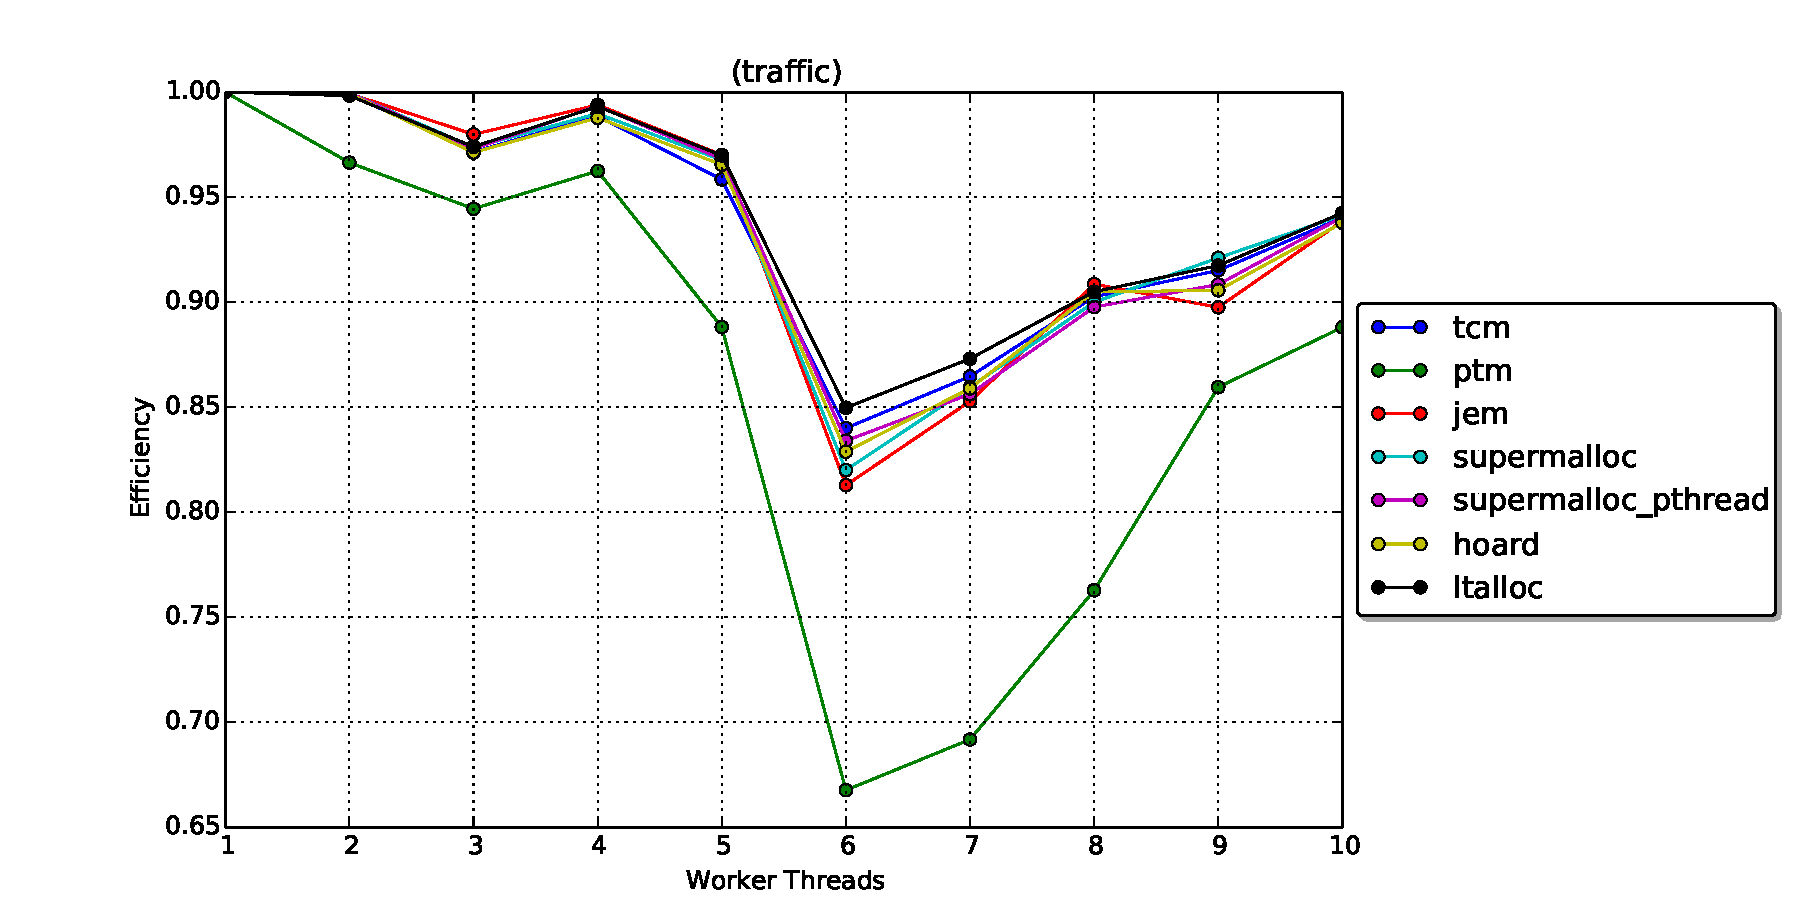
\includegraphics[width=\textwidth]{../figs/memory_allocation/traffic_efficiency.pdf} \\
        \end{column}
        \begin{column}{0.5\textwidth}
            \begin{itemize}
                \item ptmalloc2 default in GLIBC
            \end{itemize}
        \end{column}
        \end{columns}
    \end{block}
\end{frame}

\begin{frame}{Message Aggregation}
    \begin{minipage}{0.5\textwidth}
        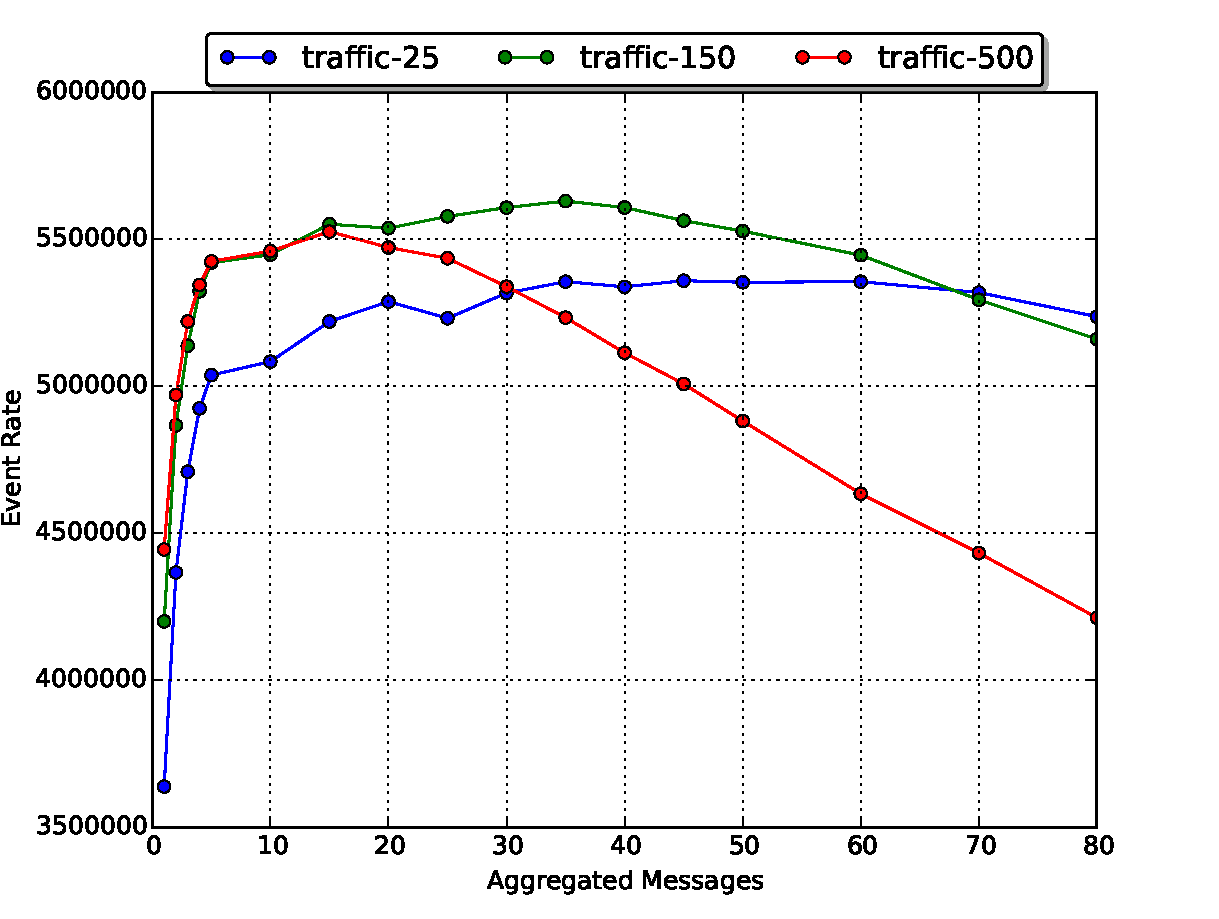
\includegraphics[width=\textwidth]{../figs/partitioning_communication/aggregate_traffic_eventrate.pdf}
    \end{minipage}%
    \begin{minipage}{0.5\textwidth}
        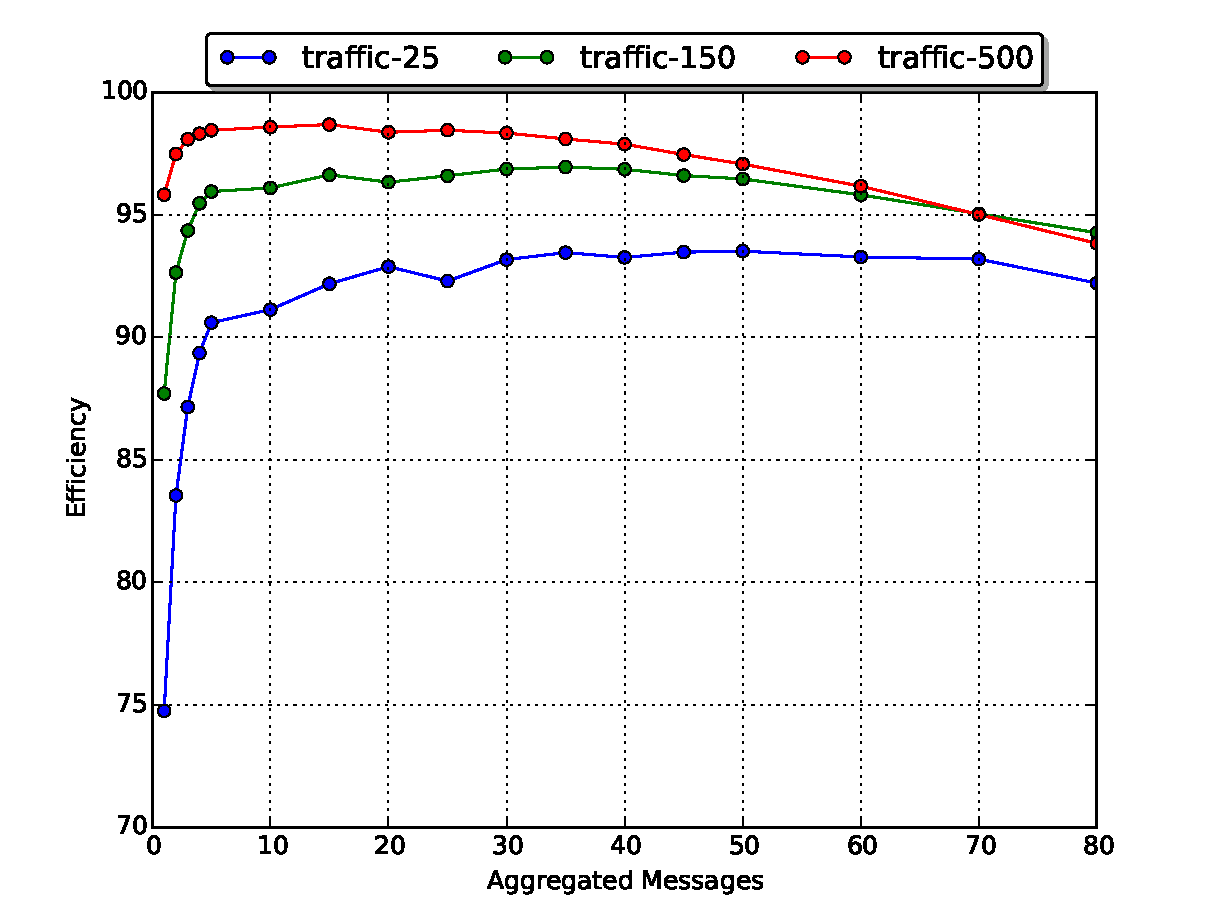
\includegraphics[width=\textwidth]{../figs/partitioning_communication/aggregate_traffic_efficiency.pdf}
    \end{minipage}   
\end{frame}

\end{document}

